\subsection{数据库索引及文件IO}
\subsubsection{数据库索引}
对于没有index的表的查询,DBMS需要将整行数据取出并在其中少数几个字段应用筛选器,这种操作是低效的。而为了能直接定位所需的记录,DBMS设计了\emph{索引}这种与文件相关联的附加的结构。常用的索引形式为B$^+$树及散列索引。
\par 当查询的限定字段被某一索引所包括时,DBMS首先查找索引,找出相应记录所在的磁盘块,再取出相应的(存储数据量较小的)磁盘块并在其中高效搜索\textsuperscript{\cite{silberschatz-2010}} 。但索引并非越多越好:一方面,创建索引和动态维护索引要耗费时间;另一方面,索引需要占物理空间,除了数据表占数据空间之外,每一个索引还要占一定的物理空间,如果要建立聚簇索引,那么需要的空间就会更大。


\par 在以下情况下使用索引能带来较优的效果\textsuperscript{\cite{silberschatz-2010}}:
\vspace{-1.5em}
\paragraph{\ding{172}} 频繁需要搜索的列;
\vspace{-1.5em}
\paragraph{\ding{173}} 主键列、唯一性约束、外键列等,强制该列的唯一性和组织表中数据的排列结构(PostgreSQL会自动为这些列设置索引);
\vspace{-1.5em}
\paragraph{\ding{174}} 连接表或检查被用作连接(join)的列,即一般指外键列;
\vspace{-1.5em}
\paragraph{\ding{175}} 经常需要进行范围搜索的列,可利用索引已排序的特性对数值进行连续搜索;
\vspace{-1.5em}
\paragraph{\ding{176}} 经常需要排序的列同样可利用索引已排序的特性减少排序步骤的耗时;
\vspace{-1.5em}
\paragraph{\ding{177}} 频繁作为限定条件的字段组合(列)。

\par 而以下情况使用索引的效果并不佳:
\vspace{-1.5em}
\paragraph{\ding{172}} 查询中很少使用或者参考的列不应该创建索引(对查询速度的优化场景较少,而DBMS多了储存与维护索引的时间、空间负担);
\vspace{-1.5em}
\paragraph{\ding{173}} 数据量较少的列不需要设置索引;
\vspace{-1.5em}
\paragraph{\ding{174}} 连接表或检查被用作连接(join)的列,即一般指外键列;
\vspace{-1.5em}
\paragraph{\ding{175}} Text, image, blob等数据类型的列不应该增加索引,因为这些列的数据量较大或取值很少;
\vspace{-1.5em}
\paragraph{\ding{176}} 需要频繁修改而较少需要检索的表:修改性能和检索性能互相矛盾,当增加索引时,会提高检索性能,但是会降低修改性能,当减少索引时,会提高修改性能,降低检索性能。\\~\\
\centerline{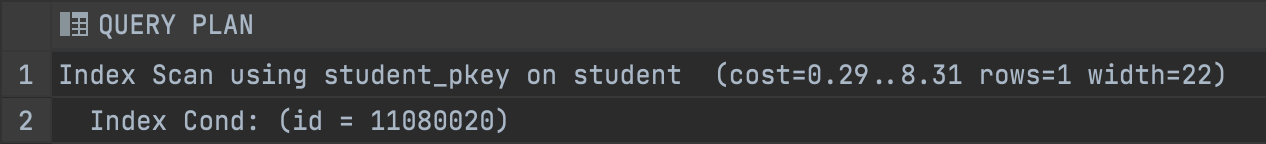
\includegraphics[width=0.6\textwidth]{sp/idx}}
\scriptsize
\centerline{SELECT * FROM project1.student WHERE id = 11080020; 这里id作为主键列已经设有index}
\normalsize

\par 以下查询所有与海洋相关的院系所开设的课程及教师。此时join中用到的连接列均有数据库默认加上的index,键入EXPLAIN ANALYSE命令分析可见大量\emph{hash join, hash cond, index scan, index cond}等,查询耗时0.368ms。
\begin{lstlisting}
SELECT c.name, t.name
FROM project1.course c
         JOIN project1.department d ON c.dept = d.id
         JOIN project1.class cls ON cls.course = c.cid
         JOIN project1.class_teacher ct ON ct.class = cls.id
         JOIN project1.teacher t ON t.id = ct.teacher
WHERE d.name ~ '海洋'
ORDER BY c.name, t.name;
\end{lstlisting}
\vspace{-2em}
\centerline{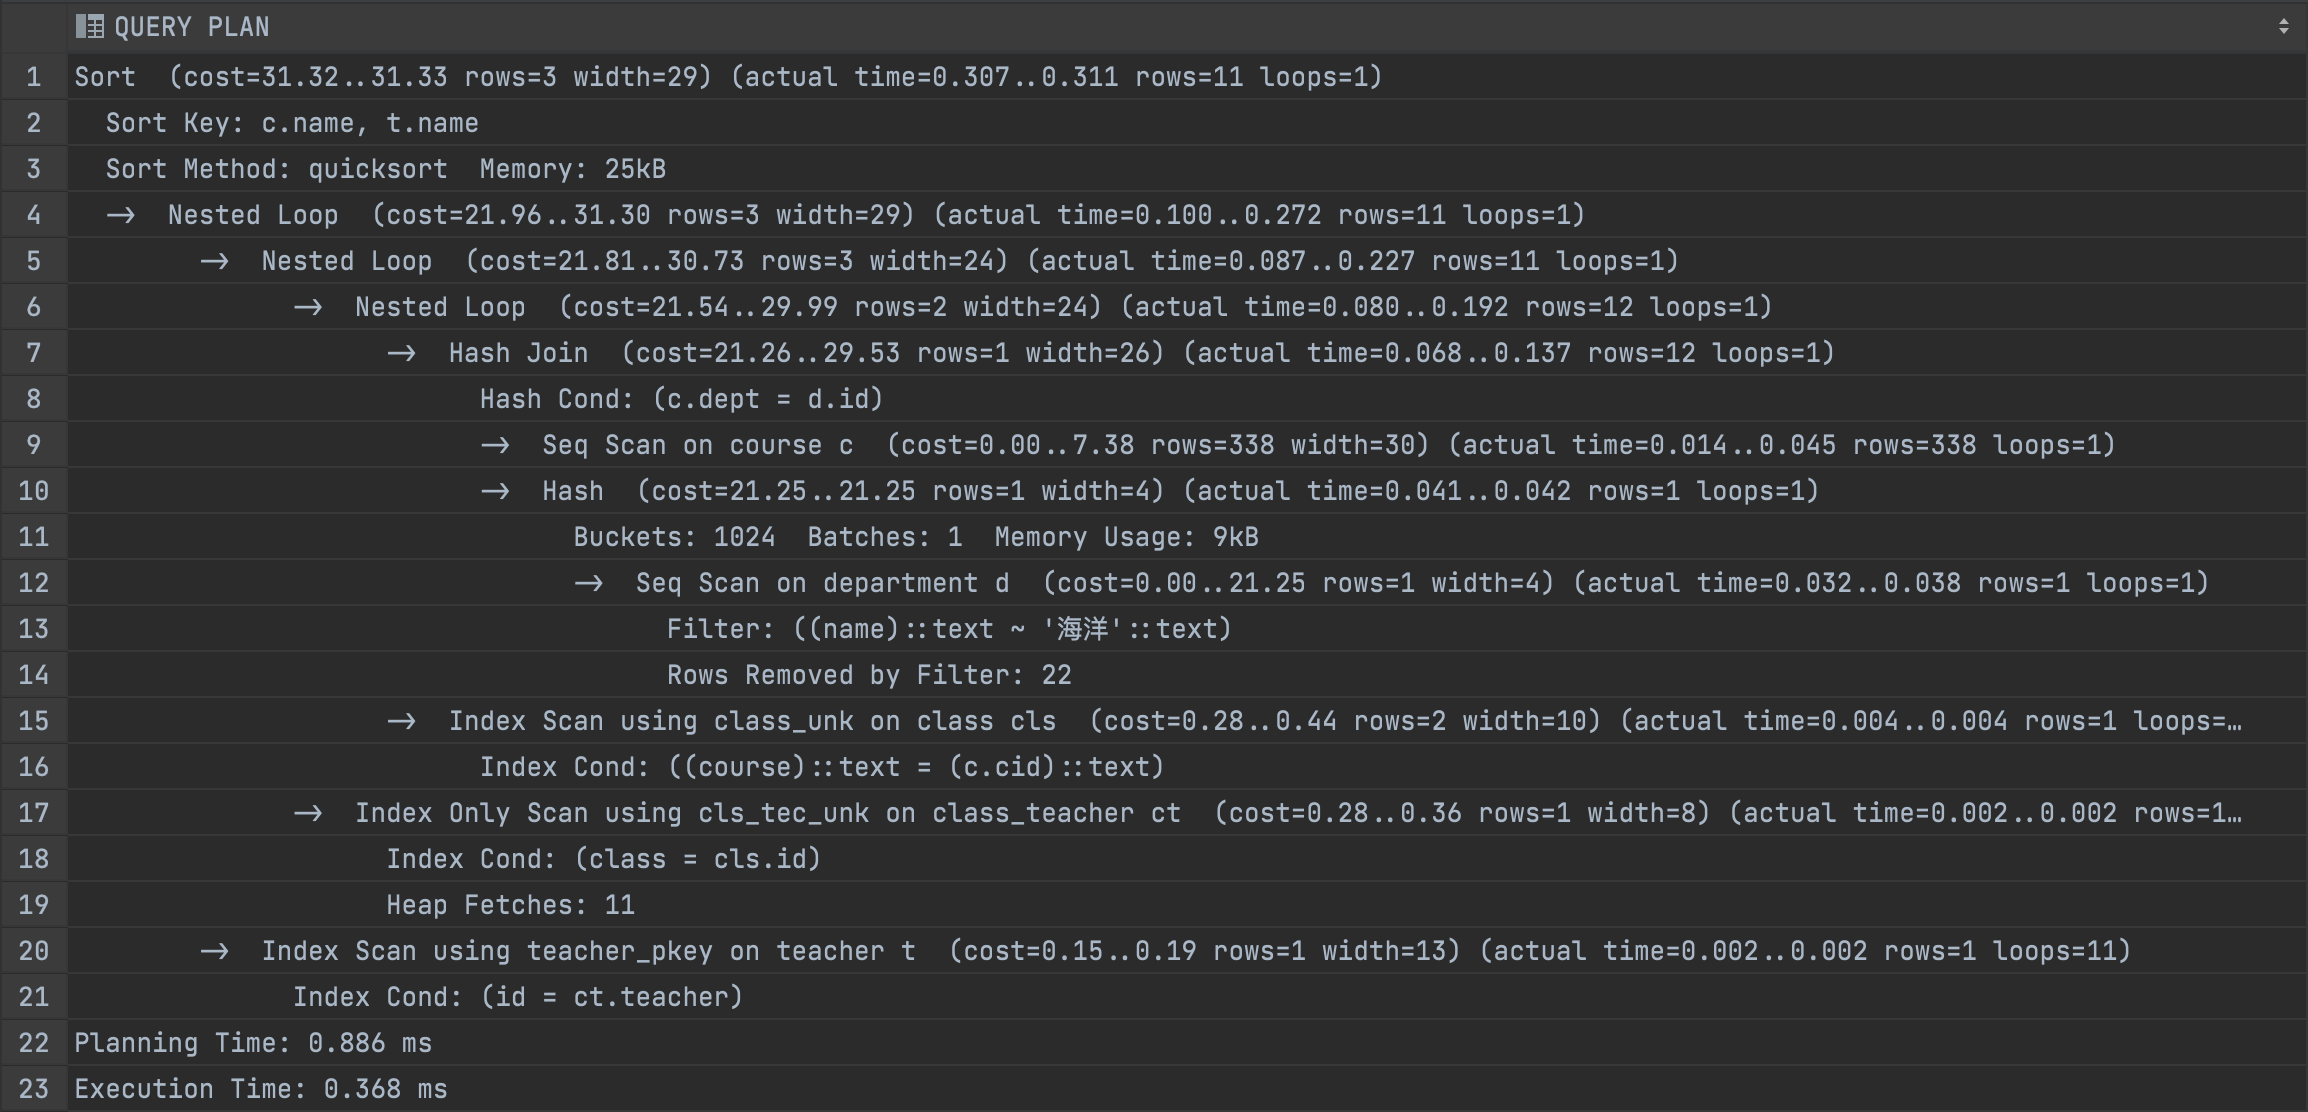
\includegraphics[width=0.85\textwidth]{sp/idxp}}

\par 下面通过对比能体现索引带来了极高的查询效率提升。对于查询语句\textbf{SELECT class FROM schedule WHERE weekday = 5},原始的无索引查询(如左下图)进行了序列扫描,需要取出表中所有信息,耗时0.281s,而通过\textbf{CREATE INDEX ON project1.schedule (weekday)}为WHERE限定列加上索引后,查询耗时仅为0.147s(如右下图),相比无索引查询节省了47.6\%的时间。\\~\\
\centerline{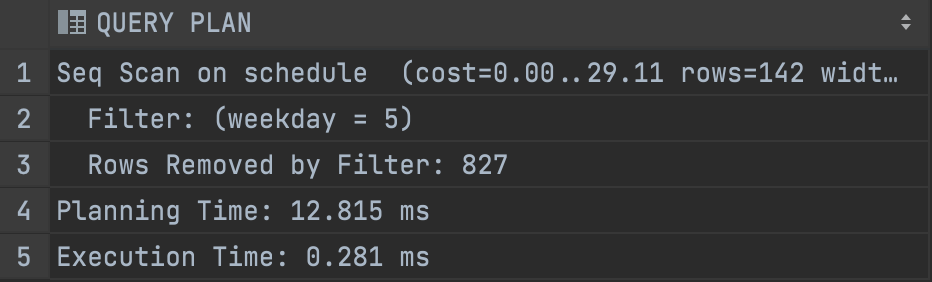
\includegraphics[height=4em]{sp/nid}\qquad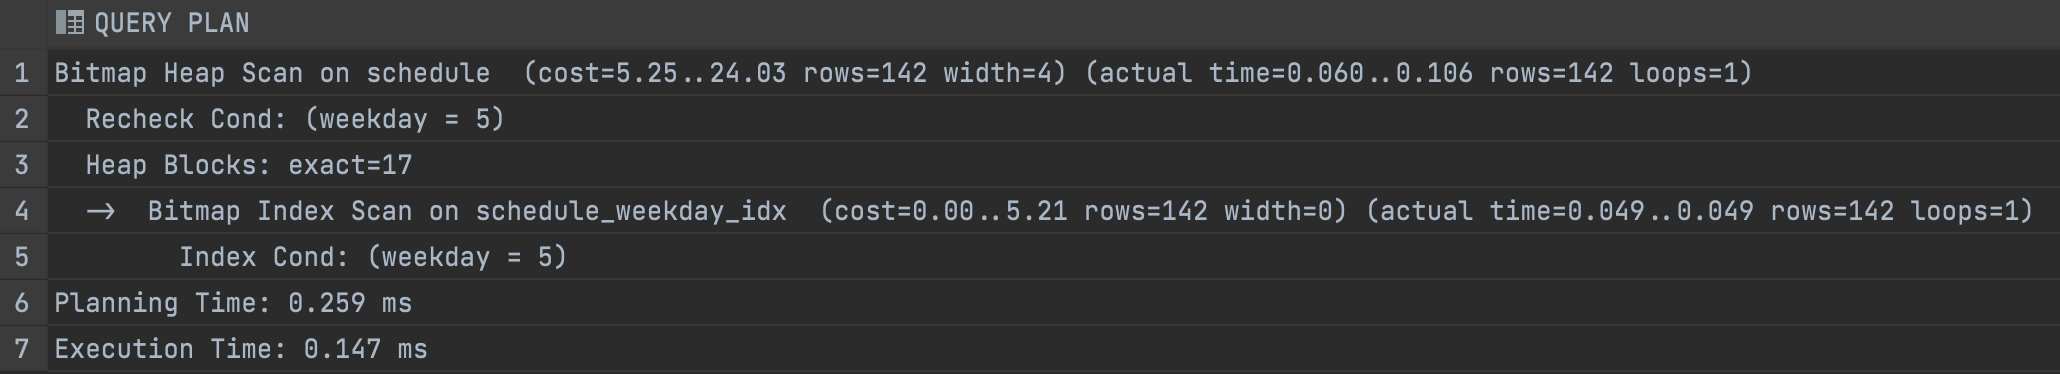
\includegraphics[height=4em]{sp/id}}

\subsubsection{文件索引(数据结构)}
使用Python对无索引的课程信息文件十次检索学分大于2的课程,耗时0.525s:
\begin{lstlisting}[language=python]
def fs_query() -> set:
    result_set = set()
    for _ in range(10):
        result_set.clear()
        for index, c in cif.iterrows():
            if c['courseCredit'] > 2:
                result_set.add(c['courseId'])
    return result_set
\end{lstlisting}
\vspace{-2em}
\par 下面为相应条目创建索引\footnote{使用了GitHub上的B+树代码实现:adigan1310 / BPlus-Tree-Indexing}\textsuperscript{\cite{unknown-author-2017}}
\begin{lstlisting}[language=java]
Index idx = new Index();
idx.index("courseCredit", "course_info.json", "idx_course_info.bpt");
idx.searchindex("idx_course_info.bpt", "courseCredit > 2", " ");
\end{lstlisting}
\vspace{-2.3em}
\par 调用该封装好的函数如同使用SQL一样方便,首先需要对对应的字段创建索引,然后解析此索引并进行搜索,并加工searchindex函数返回的原始结果(相对于 SELECT *),十次搜索耗时0.319s,但考虑到JVM和Python interpreter的性能差异,该结果仅供参考。